%!TEX root = ../main.tex

\section{Differential cross section}
\label{sec:differential-cross-section}

As a second task, the validity of the Klein-Nishina formula presented in
\autoref{eq:klein-nishina} is tested. For this purpose, the spectrometer is placed
at various angles relative to the beam path. For every angle two measurements of
\SI{300}{\second} each are taken. One measurement with a cylindrical aluminum target
in the beam path that allows for Compton scattering. The second measurement is
conducted without any target and will help quantify the background noise measured
by the spectrometer. The resulting distribution of electron energies is shown in
\autoref{fig:diff-measurements} for all measurements.

\begin{figure}
  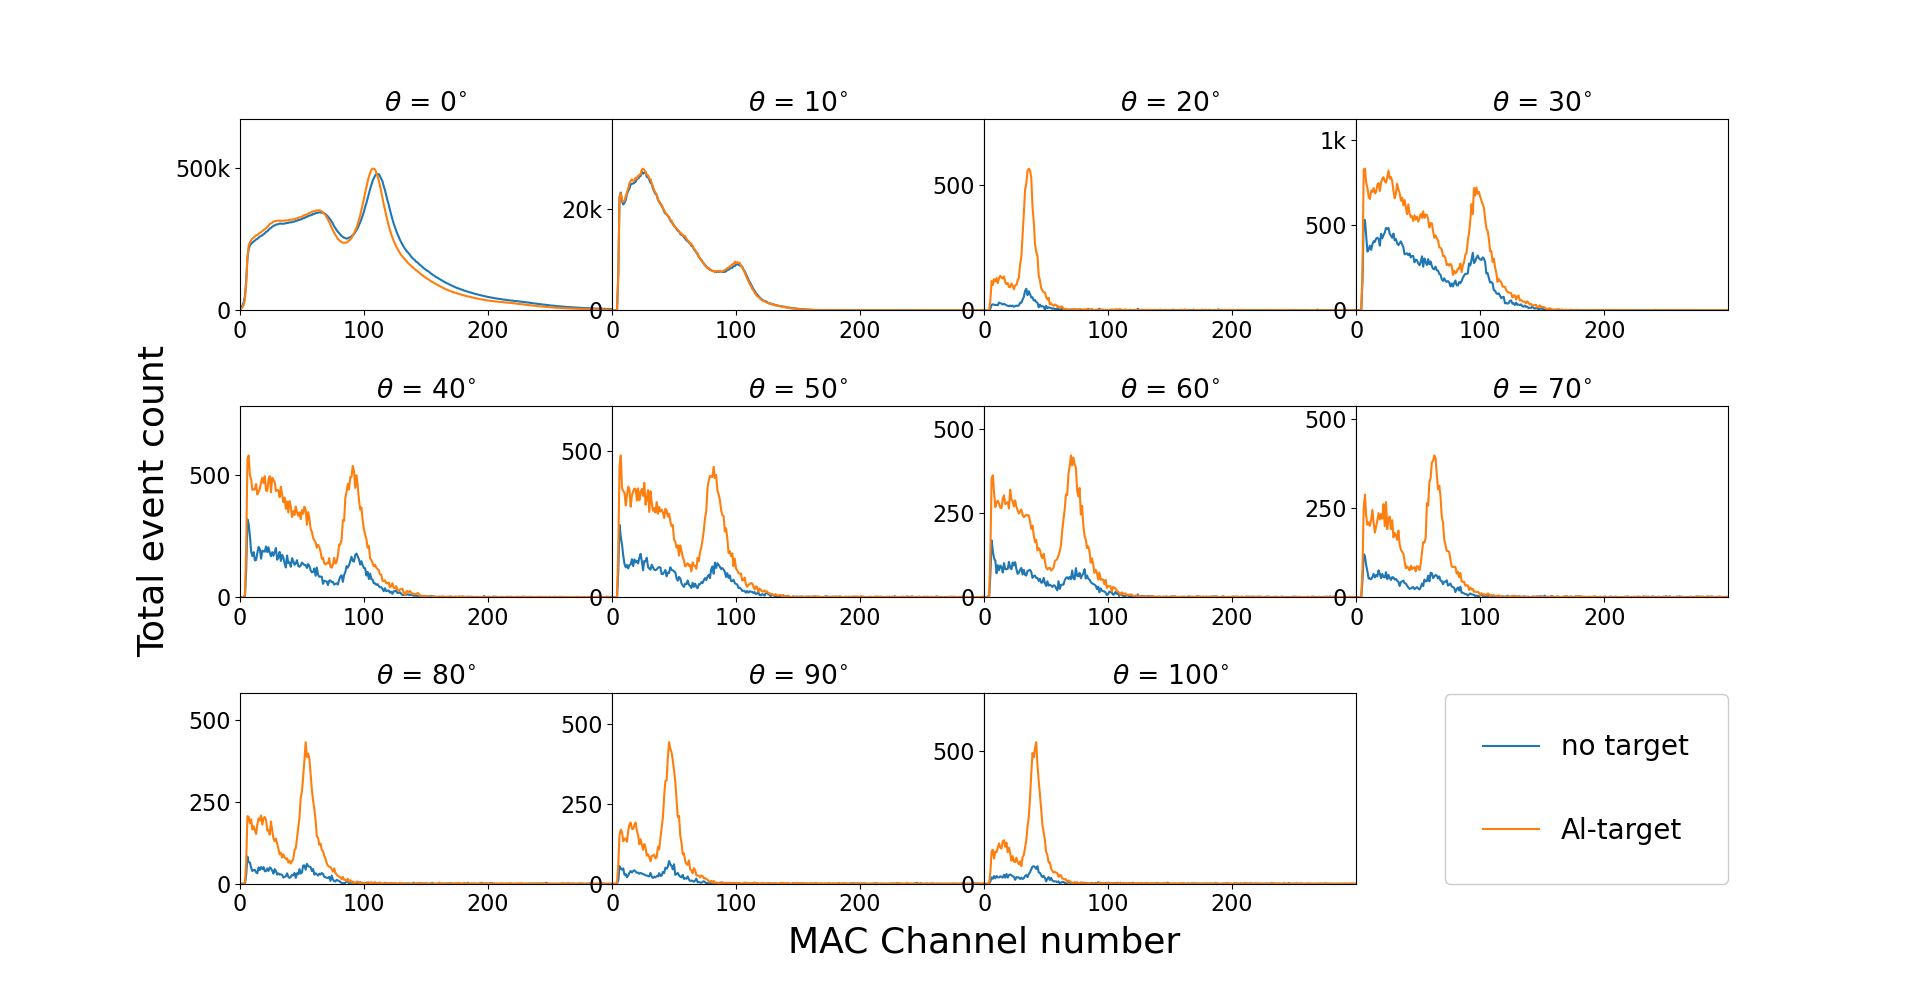
\includegraphics[width=1.0\textwidth]{./fig/differential measurements.png}
\caption{Raw number of events counted in every channel for each measured angle.
  The dashed black lines indicate the theoretical energy a photon has after
  undergoing compton scattering at an angle $\theta$. The distance between signal
  peaks and this energy grows with increasing scattering angles. This is expected
  due to the imperfect calibration.}\label{fig:diff-measurements}
\end{figure}

Before processing the data further, the abnormally high counts for the measurements
at $0$ and $10$ degrees need to be adressed. The gamma spectra look identical 
whether a target is placed in the beam path or not. In this case $\gamma$'s can 
directly propagate from the $^{137}$Cs-source to the scintillating crystal due to the
low deflection angle of the experimental setup. It is not the Compton spectrum that 
is measured at these angles, but rather the flux $\upphi_0$ of the $\gamma$ source. 
The two  measurements have to be discarded in the following analysis.

Furthermore, the detector quantum efficiency $\epsilon$ has to be evaluated. For this
purpose a second order polynomial is fitted to Plot 7.10 (p.134) in \cite{Sch17}. The
parameters of the best fit result are given below.

\begin{align*}
\label{eq:eq:efficiency-parameters}
	\epsilon(E) &= a E^2 + b E + c \\
	a &= \SI{1.77 \pm 0.1 e-6}{\per\mega\electronvolt\squared} \\
	b &= \SI{-2.340 \pm 0.087 e-3}{\per\mega\electronvolt} \\
	c &= \SI{1.252 \pm 0.017}{}
\end{align*}

In the subsequent analysis, the counts for each measured channel are normalised with
respect to the detector efficiency at the energy corresponding to the specific
channel (see \autoref{eq:ecal-eq}). The corrected count for each channel is given as 
$n_{\mathcal{C},\text{corr}}  = \frac{n_\mathcal{C}}{\epsilon( E(\mathcal{C}) )}$. 
All detector hits are then summed up and divided by the measurement length to get the
integrated rate $R$ at one specific solid angle $\Delta\Omega$ and one specific 
scattering angle $\theta$. From this, the differential cross section 
$\frac{\d\sigma}{\d\Omega}$ can be obtained as lined out in \cite{Sch17}.

\begin{equation}
\label{eq:diff-cross-section-experimental}
	\frac{\d\sigma}{\d\Omega} = \frac{R(\Delta\Omega,\theta)\,_\text{Sig}\;-R(\Delta\Omega,\theta)\,_\text{Bkg}}{\Delta\Omega \cdot \upphi_0 \cdot n_e},
\end{equation}

where $\Delta\Omega$ is the solid angle covered by the scintillator detecor as seen
from the target position. $\upphi_0$ is the flux of photons hitting the target. $n_e$
holds information about the number of scattering partners (i.e. electrons) available
to a single photon. With information given in \cite{Sch17} their numerical value can 
be calculated as shown below. Note that in order to quantify errors in the mentioned 
variables, all information given by \cite{Sch17} is assumed to be exact.

\begin{align*}
	\Delta\Omega &= \SI{0.01105 \pm 0.0}{\steradian} \\
	\upphi_0 &= \SI{4.956 \pm 0.290 e9}{\per\meter\squared\per\second} \\
	n_e &= \SI{6.153 \pm 0.688 e23}{} \\
\end{align*}

Assuming a poissonian error $\Delta N = \sqrt{N}$ for each channel, as well as
neglecting any possible correlation, \autoref{eq:diff-cross-section-experimental}
holds an uncertainty $\Delta S$, which propagates like

\begin{equation}
\label{eq:cross-section-error}
	\Delta S = \sqrt{ \left(\frac{\Delta R(\Delta\Omega,\theta)}{\Delta\Omega\upphi_0 n_e} \right)^2 + \left(\frac{R(\Delta\Omega,\theta)}{\Delta\Omega\upphi_0 n_e}\;\cdot\;(\frac{\Delta\upphi_0}{\upphi_0} + \frac{\Delta n_e}{n_e} ) \right)^2 }
\end{equation}

\begin{figure}
	\centering
	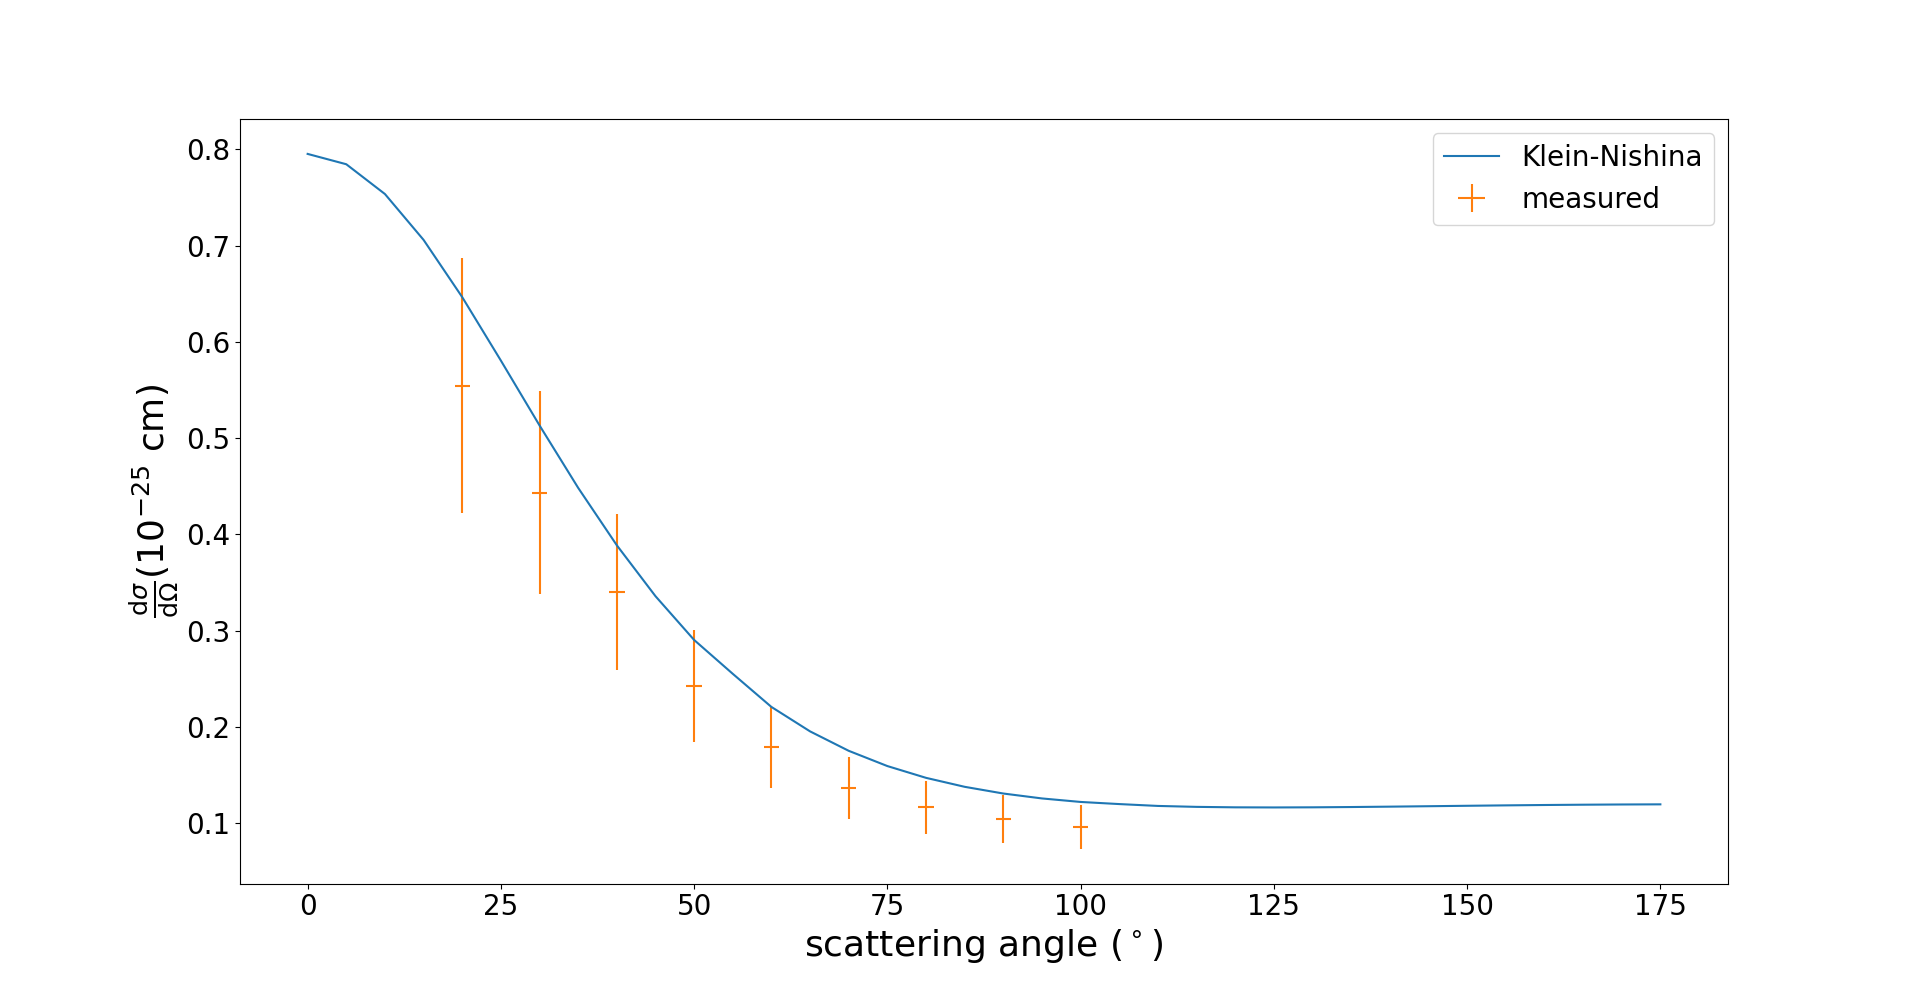
\includegraphics[width=1.0\textwidth]{./fig/differential-cross-section.png}
	\caption{The experimentally measured differential cross section is compared
	to the theoretically predicted values given by the Klein-Nishina formula.
	While the gathered data is in good accordance with the theory, the measured
	values are offset by a constant. This indicates the presence of systematic
	errors.}
	\label{fig:diff-cross-section}
\end{figure}

The results of this analysis are presented in \autoref{fig:diff-cross-section}. They
withstand the comparison to theoretical values given by \autoref{eq:klein-nishina}.
Worrysome is however a constant offset by which the measurements deviate from
theoretical data. The offset indicates the presence of systematic errors in the
experiment. One certain error source may be the imperfect energy-channel calibration
discussed in \autoref{sec:ecal}.
